\documentclass{beamer}
\usepackage[en]{zafu}
% Charts on slides
\usepackage{pgfplots}
\pgfplotsset{compat=1.17}
% Rules for tables
\usepackage{booktabs}

% PDF metadata and safe bookmark settings (no visual changes)
\hypersetup{
  pdftitle={An Informer-Based Calibration-Free LIBS Spectral Identification},
  pdfauthor={Birrul Walidain; Nasrullah Idris; Khairun Saddami; Natasya Yuza},
  pdfsubject={LIBS; Informer; Calibration-free; Spectral Analysis},
  pdfkeywords={LIBS, Informer, Spectral Identification}
}
% Avoid warnings from superscripts and line breaks in PDF strings
\pdfstringdefDisableCommands{%%
  \def\\{}%% ignore manual line breaks in bookmarks
  \def\textsuperscript#1{#1}%% drop superscript styling in bookmarks
}

% Metadata (7-minute presentation)
\title[Calibration-Free LIBS w/ Informer]{An Informer-Based Calibration-Free LIBS Spectral Identification}
\subtitle{Case Study: Emission Spectra of Aceh Traditional Women's Medicine}
\author[Walidain et al.]{
  Birrul Walidain\textsuperscript{1}, Nasrullah Idris\textsuperscript{1*}, \\
  Khairun Saddami\textsuperscript{2}, Natasya Yuza\textsuperscript{1}
}
\institute{
  \small
  \textsuperscript{1}Department of Physics, Faculty of Mathematics and Natural Sciences\\
  \textsuperscript{2}Department of Electrical and Computer Engineering\\
  \textbf{Universitas Syiah Kuala}, Banda Aceh, Indonesia, 23111\\
  \vspace{0.5em}
  \textsuperscript{*}Corresponding author: \texttt{nasrullah.idris@usk.ac.id}
}
\date{September 5, 2025}

% Optional: small logo on title (uses your USK logo)
\titlegraphic{\includegraphics[width=0.16\textwidth]{src/logo-usk.png}}

\begin{document}

% Slide 1: Title Slide (0:00–0:30)
\maketitle

\section{Introduction}

% Slide 2: Research Objectives (0:30–1:15)
\begin{frame}{Research Objectives}

  \begin{block}{Main Goal}
    \centering
    To develop a calibration-free LIBS analysis method using an efficient Informer-based trained on physics-based synthetic data.
  \end{block}

  \vspace{0.6em}

  	\textbf{Our Approach in 3 Steps:}
  \begin{enumerate}\setlength{\itemsep}{2pt}\setlength{\parskip}{0pt}
    \item \textbf{Simulate:} We generate a large, physics-based spectral library from Saha Boltzmann Equations \& National Institute of Standards and Technology (NIST) Atomic Spectra Database (ASD) atomic transition data, completely eliminating the need for expensive experimental calibration.
    \item \textbf{Analyze:} We use an efficient Informer model a first for LIBS to rapidly analyze high resolution spectra and deconvolve complex multi-element signals.
    \item \textbf{Validate:} We prove the method's real-world viability by successfully identifying key elements in complex traditional medicine samples.
  \end{enumerate}
\end{frame}

% Slide 3: Problem Statement (1:15–1:45)
\begin{frame}{Why LIBS Analysis is Challenging}
  \begin{columns}[T,onlytextwidth]
    \begin{column}{0.75\textwidth}
      \vspace{0pt}
  \includegraphics[width=\linewidth,height=0.9\textheight,keepaspectratio]{gallery/slide/libs_4panel.png}
    \end{column}
    \begin{column}{0.26\textwidth}
      \vspace{0pt}
      {\scriptsize
      	\textbf{LIBS spectral challenges:}
      \begin{itemize}\setlength{\itemsep}{0pt}\setlength{\parskip}{0pt}
        \item Line overlap and interference
        \item Self-absorption and broadening
        \item Continuum background and shot-to-shot noise
        \item Matrix effects; $T$ and $n_e$ variations
      \end{itemize}
      Panels: Pure Spectra: Fe, Ti, Ca (a) Combined Spectra T=8000K (b) Components vs Mixture (c) Impact of Temperature Variability on Spectrum (d)}
    \end{column}
  \end{columns}
\end{frame}

\section{Methodology}

% Slide 4: Informer Architecture (1:45–2:30)
\begin{frame}{Informer-Based Solution}
  \begin{block}{Key Innovation: ProbSparse Self-Attention}
    Scale: High-resolution spectra → Complexity reduced from $\mathcal{O}(L^2)$ to $\mathcal{O}(L \log L)$; focuses on the most informative channels.
  \end{block}

  \vspace{0.1em}

  \begin{columns}[T]
    \begin{column}{0.80\textwidth}
        \textbf{Core Method (Problem $\rightarrow$ Solution):}
      \begin{itemize}\setlength{\itemsep}{1pt}
        \item \textbf{Problem}: High data scale $\rightarrow$ \textbf{Solution}: ProbSparse Self-Attention for fast and efficient analysis.
        \item \textbf{Problem}: Model complexity $\rightarrow$ \textbf{Solution}: A 2-layer encoder provides the best trade-off between accuracy and generalization (avoids overfitting).
        \item \textbf{Problem}: Weak signals $\rightarrow$ \textbf{Solution}: \textit{MultiLabelFocalLoss} emphasizes minority signals for higher sensitivity.
        \item \textbf{Output}: Multi-label classification of 18 elements from a single spectrum.
      \end{itemize}

      \vspace{0.25em}
    \end{column}
    \begin{column}{0.25\textwidth}
      {\centering \includegraphics[width=\linewidth,height=0.9\textheight,keepaspectratio]{images/3-Arsitektur-Informer.drawio.pdf}\\}
    \end{column}
  \end{columns}

\end{frame}
% Slide 5: Dataset and Training (2:30–3:15)
\begin{frame}{Physics-Based Synthetic Training}
  \begin{block}{Synthetic Spectra Library (Calibration-Free)}
    Build a large synthetic spectra library to train the model without scarce and expensive calibrated data
  \end{block}

  \begin{columns}[T]
    \begin{column}{0.8\textwidth}
      	\textbf{Core Method (Problem → Solution):}
      \begin{itemize}\setlength{\itemsep}{1pt}
        \item \textbf{Problem}: training a model needs a large and diverse spectral library; calibrated experimental data is expensive
        \item \textbf{Solution}: build a “virtual library” of 50{,}000 synthetic spectra  → fully calibration-free
        \item \textbf{Saha–Boltzmann equations}: compute spectral intensities under varying plasma conditions (T, $n_e$)
        \item \textbf{NIST Atomic Spectra Database (ASD)}: use gold-standard atomic transition data source
        \item \textbf{Realistic complexity}: model multi-element interference and line broadening
      \end{itemize}
    \end{column}
    \begin{column}{0.2\textwidth}
      \centering
      \includegraphics[width=\linewidth,height=0.7\textheight,keepaspectratio]{gallery/slide/Physics-d.png}
    \end{column}
  \end{columns}
\end{frame}

\section{Results}
% Slide 6: Performance Results (3:15–4:15)
\begin{frame}{Experimental Results}
  \begin{block}{Key Findings}
    High recall (0.77) shows excellent sensitivity; lower precision indicates interference challenges -- consistent with physics expectations.
  \end{block}
  \vspace{0.1em}

  \begin{columns}[T,onlytextwidth]
    \begin{column}{0.63\textwidth}
      \begin{tikzpicture}
        \begin{axis}[
          title={Model Performance (F1-Score per Element)},
          xbar,
          width=\linewidth,
          height=0.58\textheight,
          xmin=0, xmax=1.0,
          xlabel={F1-Score},
          symbolic y coords={Si,Cr,Ca,Al,Co,Fe},
          ytick=data,
          ytick style={draw=none},
          nodes near coords={\pgfmathprintnumber[fixed,precision=4]{\pgfplotspointmeta}},
          nodes near coords style={font=\scriptsize, anchor=west},
          point meta=x,
          bar width=8pt,
          enlarge y limits=0.25,
          xmajorgrids,
          grid style={gray!30},
          tick align=outside,
          tick style={black},
          ylabel style={align=center},
          yticklabel style={font=\footnotesize},
          xlabel style={font=\footnotesize},
        ]
          % Data ordered from highest (top) to lowest (bottom)
          \addplot+[draw=none, fill=gray!55] coordinates {
            (0.8397,Si)
            (0.8392,Cr)
            (0.8065,Ca)
            (0.6665,Al)
            (0.2953,Co)
            (0.1761,Fe)
          };
        \end{axis}
      \end{tikzpicture}
    \end{column}
    \begin{column}{0.40\textwidth}
      {\scriptsize
        \textbf{Average Metrics (Optimal Model):}
      \begin{itemize}\setlength{\itemsep}{2pt}\setlength{\parskip}{0pt}
        \item \textbf{Recall (0.7733): High sensitivity.} The model is excellent at finding elements that are truly present.
        \item \textbf{Precision (0.5938): Moderate selectivity. }This reflects the physical difficulty of distinguishing highly overlapping signals, which causes some false positives.
        \item \textbf{F1-Score (0.6445): A strong overall performance,} representing the balance between sensitivity and selectivity.
      \end{itemize}
      }
    \end{column}
  \end{columns}
\end{frame}

% Slide 7
\begin{frame}{Experimental Results}

  \begin{columns}[T,onlytextwidth]
    % Left column: stacked plots
    \begin{column}{0.4\textwidth}
      \includegraphics[width=\linewidth,height=0.45\textheight,keepaspectratio]{gallery/slide/1-publication_plot_385-400nm.png}\\[-0.3em]

      \vspace{0.1em}

      \includegraphics[width=\linewidth,height=0.45\textheight,keepaspectratio]{gallery/slide/2-publication_plot_585-620nm.png}\\[-0.3em]
    \end{column}

    % Right column: analysis + predictions
    \begin{column}{0.6\textwidth}
      \footnotesize % Font lebih kecil agar muat

      \textbf{Manual Analysis Findings (Reference):}
      \begin{itemize}\setlength{\itemsep}{1pt}
        \item \textit{Major:} C, H, N, O
        \item \textit{Minor:} Ca, K, Mg, P
        \item \textit{Trace:} Al, Cu, Fe, Mn, Na, Rb
      \end{itemize}
      
      \vspace{0.1em}
      
      \textbf{Informer-Based Model Predictions (Automated):}
      \begin{itemize}\setlength{\itemsep}{1pt}
        \item \textit{Major:} C, N
        \item \textit{Minor:} Ca, Mg
        \item \textit{Trace:} Al, Fe, Mn, Na
      \end{itemize}
      
      \vspace{0.1em}
      
      \begin{block}{Key Finding: High Concordance}
        The Informer-Based model successfully identified the same core elemental signature as the manual analysis.  
        This high concordance on a complex, real-world sample validates the calibration-free, synthetic-only training approach.
      \end{block}
    \end{column}
  \end{columns}
\end{frame}

\section{Conclusion}

\begin{frame}{Conclusion}
  \small
  \begin{alertblock}{Significance \& Broader Impact}
    \begin{itemize}\setlength{\itemsep}{2pt}\setlength{\parskip}{0pt}
      \item \textbf{Democratizes Analysis}: Lowers cost and technical barriers for advanced material analysis.
      \item \textbf{Accelerates Research}: Speeds up discovery in pharmacy, geology, and environmental science.
      \item \textbf{Creates New Diagnostics}: The AI acts as a new tool to identify subtle spectral patterns.
    \end{itemize}
  \end{alertblock}

  \vspace{0.4em}

  \begin{block}{Conclusion}
    \begin{itemize}\setlength{\itemsep}{2pt}\setlength{\parskip}{0pt}
      \item Introduced a calibration-free LIBS pipeline using an Informer trained on physics-based synthetic spectra.
      \item Achieved strong performance across 18 elements (Recall 0.77, F1 0.64) and high concordance on real samples.
      \item Reduced reliance on costly calibrations while remaining sensitive to overlapping and weak spectral lines.
    \end{itemize}
  \end{block}

\end{frame}

% New slide: Limitations & Future Directions
\begin{frame}{Limitations \& Future Directions}
  \begin{columns}[T,onlytextwidth]
    \begin{column}{0.5\textwidth}
      \begin{alertblock}{Limitations}
        \begin{itemize}\setlength{\itemsep}{2pt}\setlength{\parskip}{0pt}
          \item \textbf{Spectral Interference}: Overlapping lines and matrix effects can lower precision on complex mixtures.
          \item \textbf{Synthetic-to-Real Gap}: Performance may vary across instruments and plasma conditions beyond training coverage.
          \item \textbf{Background Sensitivity}: Baseline variations and self-absorption require robust pre-processing.
        \end{itemize}
      \end{alertblock}
    \end{column}
    \begin{column}{0.5\textwidth}
      \begin{exampleblock}{Future Directions}
        \begin{itemize}\setlength{\itemsep}{2pt}\setlength{\parskip}{0pt}
          \item \textbf{Expand Coverage}: Grow the spectral library (elements, ranges, T, $n_e$) for broader generalization.
          \item \textbf{Enable Quantification}: Extend from presence/absence to concentration estimation.
          \item \textbf{Real-Time Tooling}: Build an interactive, user-friendly on-site analysis application.
        \end{itemize}
      \end{exampleblock}
    \end{column}
  \end{columns}
\end{frame}
% Slide 9: Q&A and Acknowledgments (6:15–7:00 + 3 min Q&A)
\begin{frame}{}
  \centering
  \vspace{0.5em}
  {\Huge \textcolor{uskGold}{\textbf{Thank You!}}}

  \vspace{0.6em}
  {\Large Questions \& Discussion}

  \vspace{1.0em}
  {\large \textcolor{uskGold}{\textbf{Contacts:}}}\\[0.3em]
  {\small
    	extbf{Nasrullah Idris:} \texttt{nasrullah.idris@usk.ac.id}\\
    	extbf{Birrul Walidain:} \texttt{birrul@mhs.usk.ac.id}
  }

  \vfill
  {\footnotesize \textcolor{gray}{\textbf{Acknowledgments}}}\\[0.2em]
  {\scriptsize \textcolor{gray}{This research was supported by BRIN High Performance Computing (Proposals 224246 \& 189541) and LPPM USK (Patent Application S00202506246). Thanks to AIC-SE USK organizing committee.}}
\end{frame}

% Slide 10: Template Credits
\begin{frame}{}
  \vfill
  \begin{center}
    {\Large \textcolor{uskGold}{\textbf{Template Credits}}}
    
    \vspace{1.5em}
    
    {\large Presentation template based on:}
    
    \vspace{1em}
    
    {\LARGE \textbf{ZAFU Beamer Theme}}\\
    \vspace{0.5em}
    {\normalsize Original by: \textcolor{gray}{github.com/ke1ewang/ZAFU-Beamer-Theme}}
    
    \vspace{1.5em}
    
    {\large \textcolor{uskGold}{\textbf{USK Adaptation}}}\\
    \vspace{0.5em}
    {\normalsize Adapted \& Modified by: \textbf{Birrul Walidain}}\\
    {\small \textcolor{gray}{Department of Physics, USK}}
    
    \vspace{1em}
    
    {\small \textcolor{gray}{September 2025}}
  \end{center}
  \vfill
\end{frame}

\end{document}
